\documentclass[12pt,
    brazil,			% extra idiom for hyphenation
	english,        % main idiom of the document
	]{article}
\usepackage[utf8]{inputenc}
\usepackage{graphicx}
\usepackage{verbatim} % for block comments
\usepackage[hyphens]{url}
\usepackage[colorlinks=true, allcolors=black]{hyperref}
\usepackage{amsmath} % for using alignat command

\usepackage{subcaption}
\usepackage{booktabs}
\usepackage{multirow}

%% Sets page size and margins
\usepackage[a4paper,top=3cm,bottom=3cm,left=3cm,right=3cm,marginparwidth=1.75cm]{geometry}

%% Reconfigure table and figure separator
\captionsetup[table]{labelsep=period}
\captionsetup[figure]{labelsep=period}

\title{Humpback Whale Identification\\Data Analysis}
\author{Henrique Simões}

\begin{document}

\maketitle

\section{Introduction}

This report brings an overview analysis of the data used by competitors as way of training and testing the algorithms created to solve the problem of identifying humpback whales by their tail~\cite{kaggle2019humpback}. The aspects considered in this analysis are mostly the distribution of the examples over the whales' classes (i.e. number of pictures for each individual whale), the image format and properties, and issues with non-standardized images, photograph angle and occlusion.

\section{Dataset}

The competition dataset contained thousands of images of humpback whales flukes, with each of them being manually labeled with an ID by researchers. The data was divided in two parts: one for training the machine learning algorithm and another for testing it. Thus, it was required to competitors to deal only with the training data in order to develop their solutions and use the test data only for submitting the results. See table \ref{tab:number-examples} for the exact number of images in each of those datasets.

\begin{table}[hbt]
    \centering
    \setlength{\tabcolsep}{25pt} % Default: 6pt
    \renewcommand{\arraystretch}{1.5} % Default: 1
    \begin{tabular}{ccc}
        \hline \hline
        Dataset     & Number of examples    & Percentage \\ \hline
        Train       & 25361                 & 76.11 \\
        Test        & 7960                  & 23.89 \\ \hline
        Total       & 33321                 & 100.00 \\
        \hline \hline
    \end{tabular}
    \caption{Number of examples per dataset and its corresponding percentage of all data points.}
    \label{tab:number-examples}
\end{table}

All information collected throughout this report was obtained through data provided by the \textit{Kaggle} platform, such the image files themselves and the training data labels.

\subsection{Training examples distribution over the classes}

In order to have an understanding of the examples distribution over the classes, it was used the labels available for the training data points, which contained the correspondence of image files and the class they belong to. This way the number of times a given whale ID appeared in the labeling gives directly the number of examples available for that whale. Having this information available, it was possible to obtain the number of occurrences of the number of examples per class (see Table \ref{tab:occurrences-examples}).

Even though there was a reasonable number of examples for training and testing, the training dataset didn't have the same number of examples for each whale. Probably the same occurred with the testing dataset. Moreover, there were considerably more data points for some whales than others. Around 87.3\% of the whales in the training dataset had less than six photographs, and 41.4\% had only a single image for its identification (see Figure \ref{fig:frequency-examples}). Besides that, around 38.1\% of the images are pictures of unlabeled whales, collectively classified with the \textit{new\_whale} tag. 

\begin{table}[htb]
    \centering
    \setlength{\tabcolsep}{25pt} % Default: 6pt
    \renewcommand{\arraystretch}{1.2} % Default: 1
    \begin{tabular}{cc}
        \hline \hline
        Number of examples & Occurences \\ \hline
            1 & 2073 \\
            2 & 1285 \\
            3 & 568 \\
            4 & 273 \\
            5 & 172 \\
            6 & 136 \\
            7 & 86 \\
            8 & 76 \\
            9 & 62 \\
            10 & 46 \\
            11 & 39 \\
            12 & 26 \\
            13 & 14 \\
            14 & 16 \\
            15 & 19 \\
            16 & 16 \\
            17 & 17 \\
            18 or more & 81 \\
        \hline \hline
    \end{tabular}
    \caption{Occurrences of the number of examples per whale ID available in the training set.}
    \label{tab:occurrences-examples}
\end{table}

\begin{figure}[htb]
    \centering
    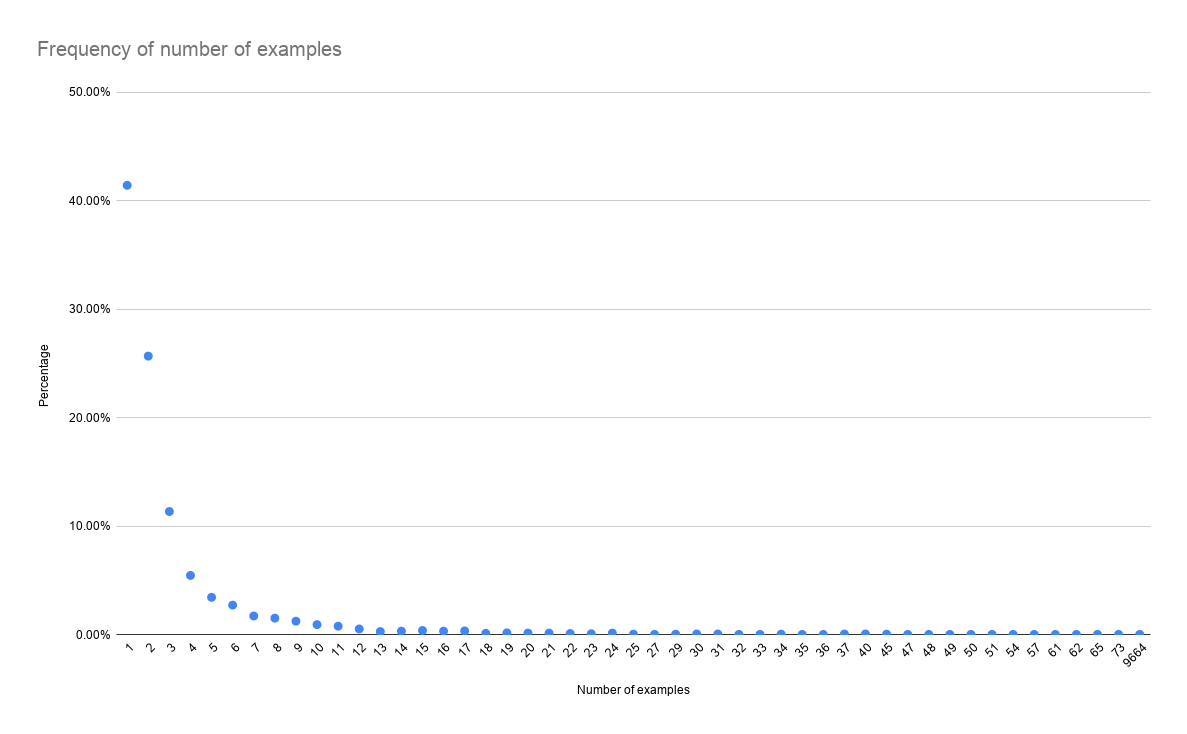
\includegraphics[width=0.95\textheight, angle=90]{images/graphs/frequency-examples.png}
    \caption{Frequency of number of examples per whale in the training dataset.}
    \label{fig:frequency-examples}
\end{figure}

\subsection{Images formats and properties}

One important aspect for building a neural network is knowing the shape of the data the network will be processing. Some image processing net architectures require a fixed size input image for being able to make a classification, such as fully connected nets. Therefore, it's useful to analyze the image size variation over the dataset, and other image properties, such as contrast, which can increase the need of the network to account for unimportant details if no normalization is done. For this part of the analysis all the examples available in both datasets were processed separately, in order to be able to identify possible differences that could challenge competitors.

\subsubsection{Images size}

Both training and testing dataset had a broad variety of image shapes, some of them being more frequent than others. Among the dataset as a whole, the most frequent image size was $1050 \times 700$ pixels. However, images with that size represent only around 13.77\% of the data points available. Other image sizes that were also more frequent are shown in Table \ref{tab:image-sizes:training} and \ref{tab:image-sizes:testing}.

\begin{table}[htb]
    \centering
    \setlength{\tabcolsep}{25pt} % Default: 6pt
    \renewcommand{\arraystretch}{1.5} % Default: 1
    \begin{tabular}{ccc}
        \hline \hline
        Height & Width & Percentage \\
        \hline
        700	&   500 &	2.63\% \\
        1050 &  450 &	6.14\% \\
        1050 &  525 &	5.14\% \\
        1050 &  591 &	1.10\% \\
        1050 &  600 &	10.05\% \\
        1050 &  700 &	13.13\% \\
        1050 &  701 &	1.04\% \\
        \hline \hline
    \end{tabular}
    \caption{Image shapes in train dataset with more than 1\% of occurrence. As it can be seen, most images had a fixed height of 1050 pixels, with a varying width size. Probably some images had a difference of a single pixel in one of its dimensions due to inaccuracy during cropping.}
    \label{tab:image-sizes:training}
\end{table}

\begin{table}[htb]
    \centering
    \setlength{\tabcolsep}{25pt} % Default: 6pt
    \renewcommand{\arraystretch}{1.5} % Default: 1
    \begin{tabular}{ccc}
        \hline \hline
        Height & Width & Percentage \\
        \hline
            700     &   500 &   1.81\% \\
            1050    &   450 &   6.58\% \\
            1050    &   525 &   5.11\% \\
            1050    &   600 &   7.89\% \\
            1050    &   700 &   15.80\% \\
            1050    &   701 &   1.87\% \\
        \hline \hline
    \end{tabular}
    \caption{Other image shapes in the test dataset and their corresponding percentage related to the total number of examples in the same dataset.}
    \label{tab:image-sizes:testing}
\end{table}

The remaining examples had dimensions varying according with the distribution shown in Figure \ref{fig:image-sizes:training} and Figure \ref{fig:image-sizes:testing}. It's notable that image width was more standardized than height. Roughly 70\% of the images had between 970 and 1150 pixels in this dimension in both training and testing set. On the other hand, the height was more distributed, ranging mostly from  200 to 900 pixels. This image ratio makes sense, once the whales' tail usually covered the image width almost entirely, having the height varying mostly because of cropping and tail angle before diving.

\begin{figure}
    \centering
    \begin{subfigure}[b]{\textwidth}
        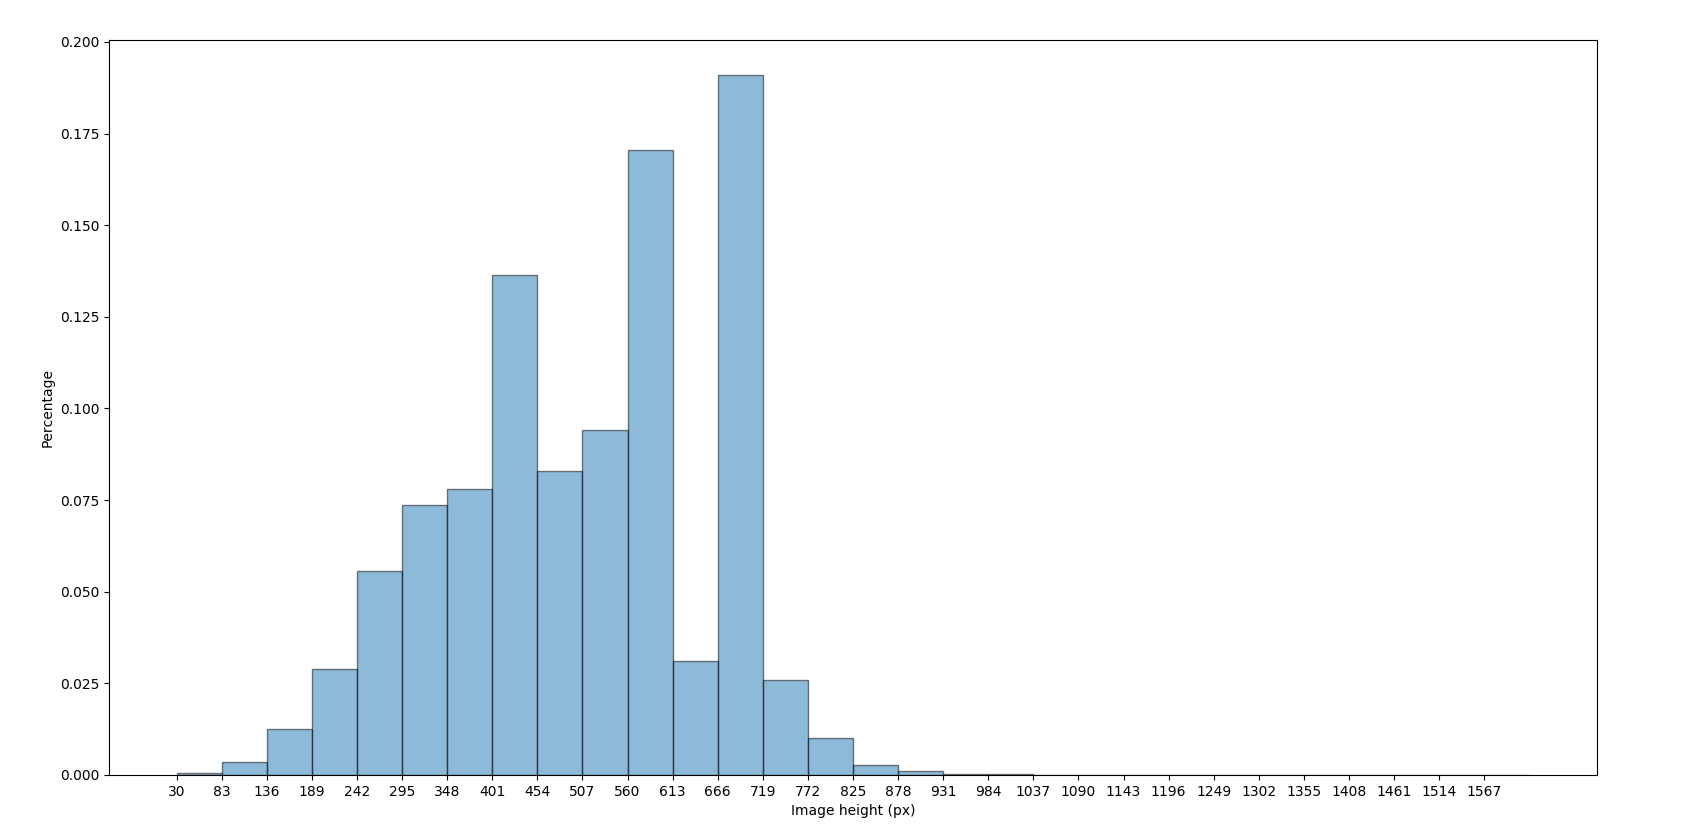
\includegraphics[width=\textwidth]{images/graphs/train-height-distribution.png}
        \caption{Image height}
    \end{subfigure}
    \hfill
    \begin{subfigure}[b]{\textwidth}
        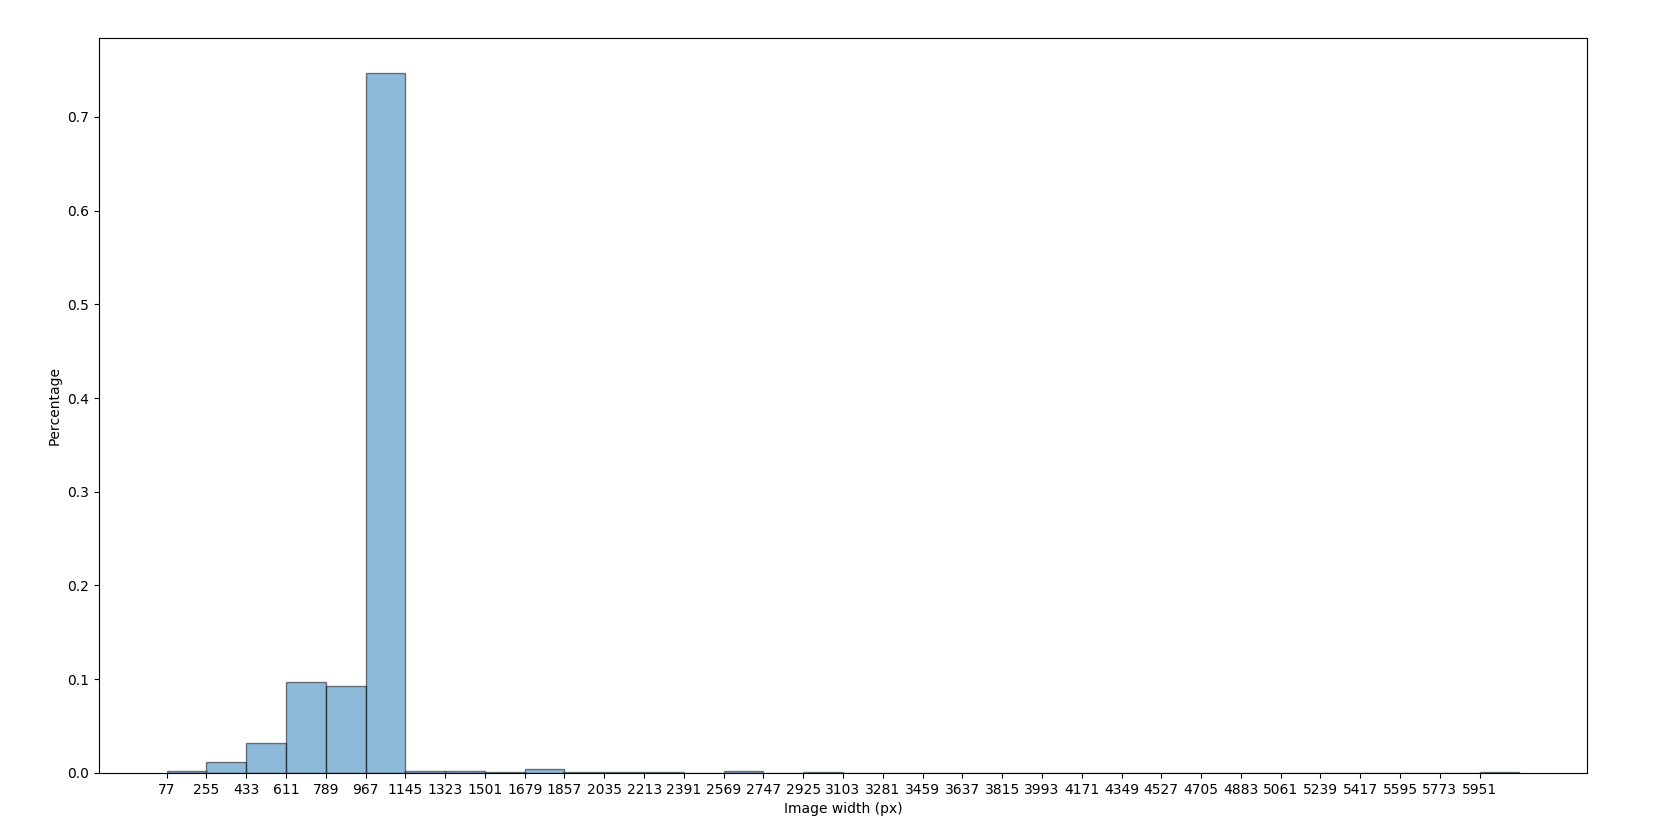
\includegraphics[width=\textwidth]{images/graphs/train-width-distribution.png}
        \caption{Image width}
    \end{subfigure}
    \caption{Image sizes distribution in the training dataset.}
    \label{fig:image-sizes:training}
\end{figure}

\begin{figure}
    \centering
    \begin{subfigure}[b]{\textwidth}
        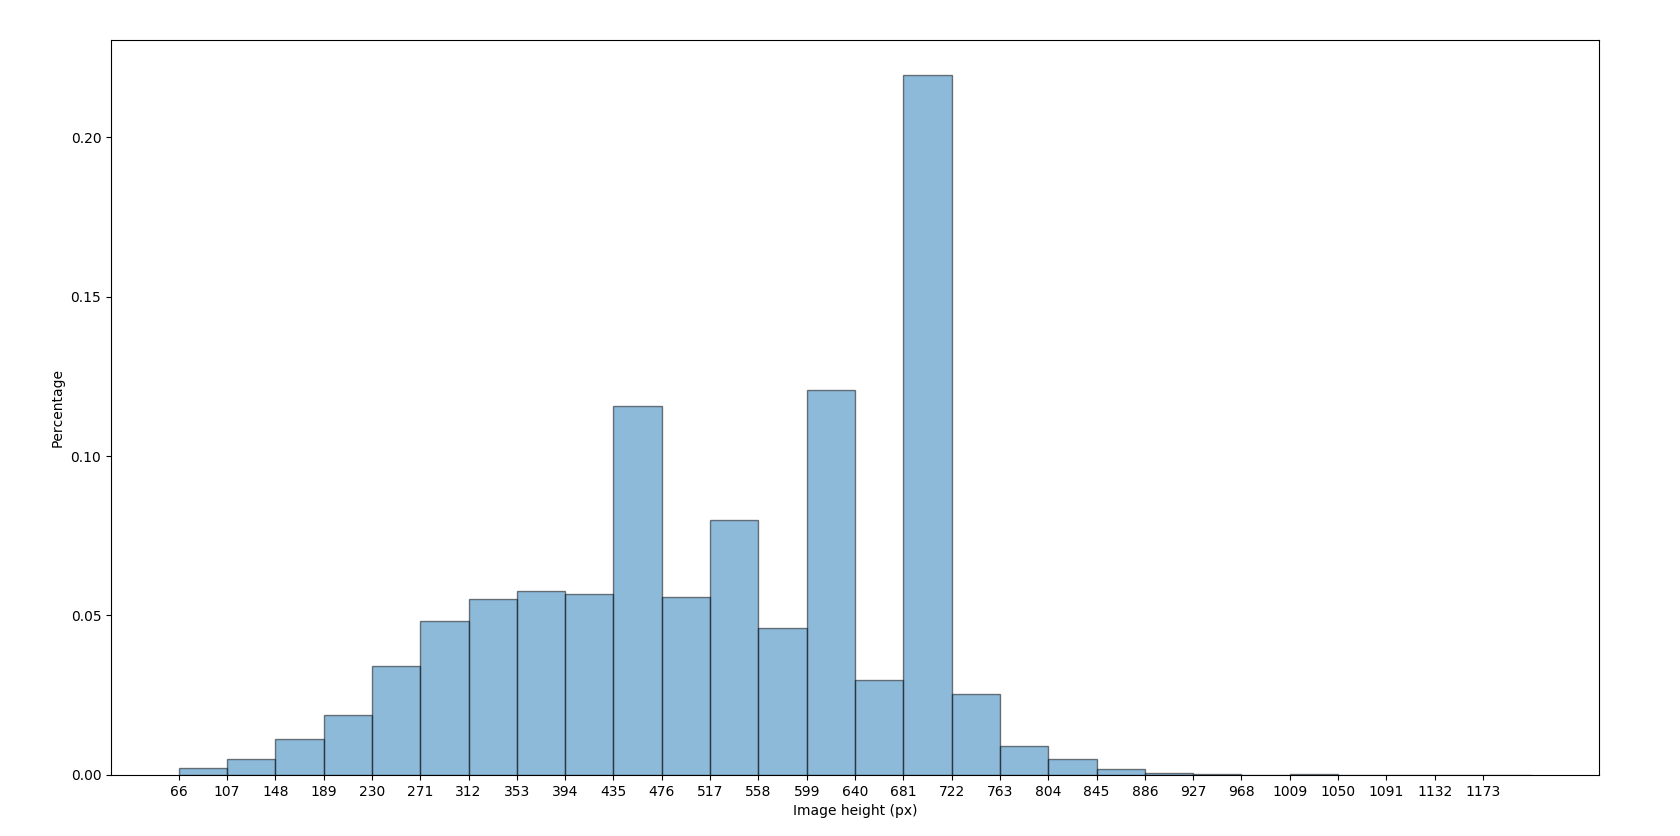
\includegraphics[width=\textwidth]{images/graphs/test-height-distribution.png}
        \caption{Image height}
    \end{subfigure}
    \hfill
    \begin{subfigure}[b]{\textwidth}
        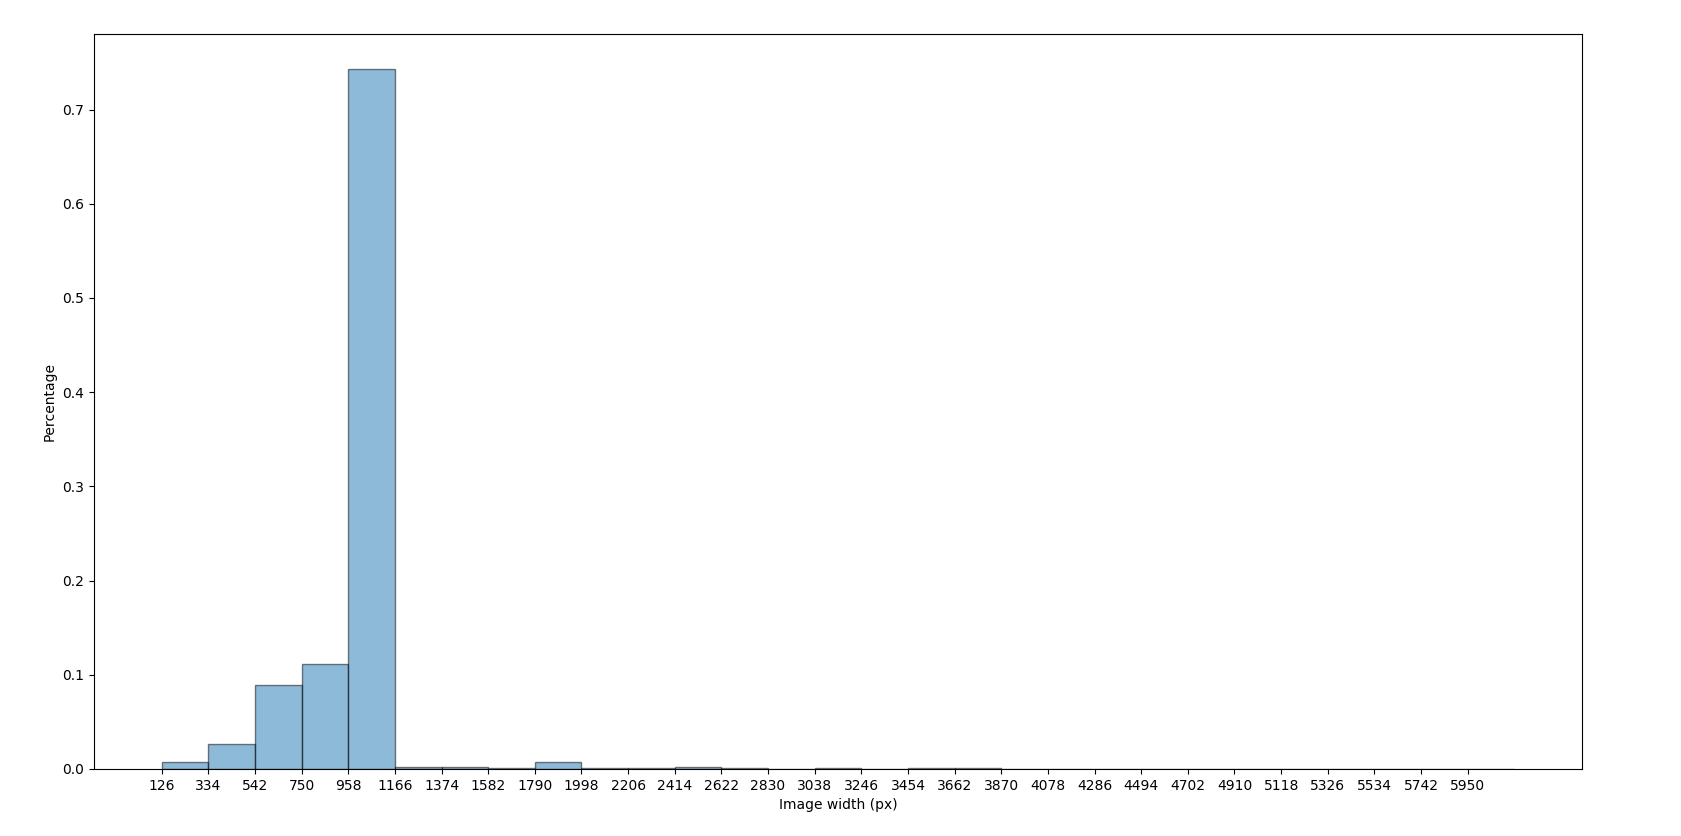
\includegraphics[width=\textwidth]{images/graphs/test-width-distribution.png}
        \caption{Image width}
    \end{subfigure}
    \caption{Image sizes distribution in the testing dataset.}
    \label{fig:image-sizes:testing}
\end{figure}

\subsubsection{Image coloring}
\label{sec:image-coloring}
Another aspect relevant for classifying images when there are few examples per class is the image coloring. Black and white images have the same information across the color channel. This means the network won't be able to use information about how different the colors intensity are in order to classify a gray scale image.

The technique used for detecting the image coloring was the usage of the \textit{Pillow} Python library~\cite{pillow2019docs} to open the image and convert it to RGB format. If the image is already in this format, nothing will be done by the function. Otherwise, i.e. the image is in gray scale, all the RGB pixels values are set to the same intensity, preserving the original image content. Once with all images in RGB format, the image will be in gray scale if, and only if, every pixel has the same intensity across all its color channels.

In the analyzed dataset, most images were colored, but nearly three tenth of the images were in gray scale (see Table \ref{tab:color}).

\begin{table}[htb]
    \centering
    \setlength{\tabcolsep}{20pt} % Default: 6pt
    \renewcommand{\arraystretch}{1.5} % Default: 1
    \begin{tabular}{*{5}{c}}
        \toprule
        \multirow{2}{*}{Dataset}    & \multicolumn{2}{c}{Gray scale}    &   \multicolumn{2}{c}{Colored} \\
        \cmidrule(r){2-3} \cmidrule(r){4-5}
                                    & Images & Percentage               & Images & Percentage \\
        \midrule
        Train                       &   8270 &  32.61\%                 &  17091 &     67.39\% \\
        Test                        &   2089 &  26.24\%                 &   5871 &     73.76\% \\
        \bottomrule
    \end{tabular}
    \caption{Number of images colored and in gray scale in the training and testing dataset and its corresponding percentage of the dataset.}
    \label{tab:color}
\end{table}

\subsubsection{Contrast}

Contrast, in the context of Deep Learning, refers to the standard deviation of the pixels in an image or region of an image~\cite{goodfellow2016deep}. In other words, the contrast in the entire image is given by
\begin{equation}
\label{eq:constrast-rgb}
    \sqrt{\frac{1}{3rc}\sum_{i=1}^{r} \sum_{j=1}^{c} \sum_{k=1}^{3} \left(X_{i,j,k} - \bar{X}\right)}
\end{equation}
where $X$ is the image represented as a tensor, with the first coordinate representing the row, the second the column and the third the color channel in RGB and $\bar{X}$ is the mean intensity of the entire image:
\begin{equation}
    \bar{X} = \frac{1}{3rc} \sum_{i=1}^{r} \sum_{j=1}^{c} \sum_{k=1}^{3} X_{i,j,k}.
\end{equation}

This information is important to be analyzed, once it may be irrelevant to the task the network is trying to perform, however the network has to discover it by itself. This is not a problem when there's a high number of examples available, but for the data available for competitors it was not the case.

In order to analyze it, the contrast was calculated for each example available in each dataset using the \textit{Numpy} Python library's~\cite{numpy2019docs} built-in algorithm for calculating standard deviation over tensors. Since gray scale images and colored images were present in both dataset, as shown in subsection \ref{sec:image-coloring}, all images were first converted to RGB color format, as described previously. Note this doesn't change the standard deviation value over gray scale images, since standard deviation across a single color dimension image (i.e. with 8-bit pixels values, black and white 'L' format) is given by
\begin{alignat}{2}
    \sigma  &= \sqrt{\frac{1}{rc} \sum_{i=1}^{r} \sum_{j=1}^{c} \left(X_{i,j} - \bar{X}\right)} \\
            &= \sqrt{\frac{1}{3rc} \sum_{i=1}^{r} \sum_{j=1}^{c} 3 \cdot \left(X_{i,j} - \bar{X}\right)} \\
            &= \sqrt{\frac{1}{3rc}\sum_{i=1}^{r} \sum_{j=1}^{c} \sum_{k=1}^{3} \left(\Tilde{X}_{i,j,k} - \bar{X}\right)}
\end{alignat}
where $\bar{X}$ is given by
\begin{alignat}{2}
    \bar{X} &= \frac{1}{rc} \sum_{i=1}^{r} \sum_{j=1}^{c} X_{i,j} \\
            &= \frac{1}{3rc} \sum_{i=1}^{r} \sum_{j=1}^{c} 3 \cdot X_{i,j} \\
            &= \frac{1}{3rc} \sum_{i=1}^{r} \sum_{j=1}^{c} \sum_{k=1}^{3} \Tilde{X}_{i,j,k}
\end{alignat}
and $\Tilde{X}$ is the image tensor representing the image after the conversion to RGB, with the original pixel value replicated over the three RGB color channels, which is exactly the same as equation \ref{eq:constrast-rgb}.

The results obtained for the images contrast is shown in Figures \ref{fig:contrast:training} and \ref{fig:contrast:testing}. It can be seen that most images had a considerably high contrast value, with a mean value of 60 pixels of contrast. This shows that candidates who applied global or local contrast normalization might have been benefited from it in their algorithm's generalization.

\begin{figure}[htb]
    \centering
    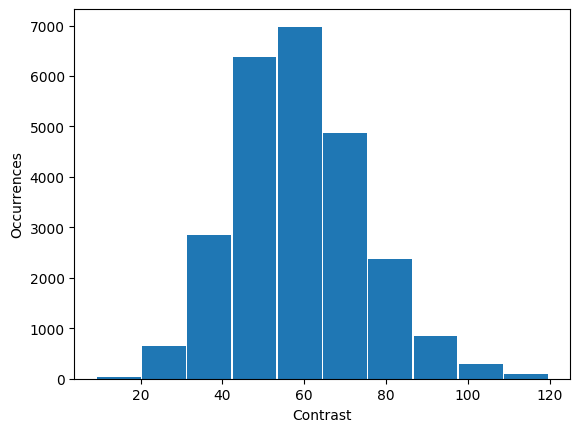
\includegraphics{images/graphs/train-contrast-hist.png}
    \caption{Contrast distribution of the images in the train dataset.}
    \label{fig:contrast:training}
\end{figure}

\begin{figure}[htb]
    \centering
    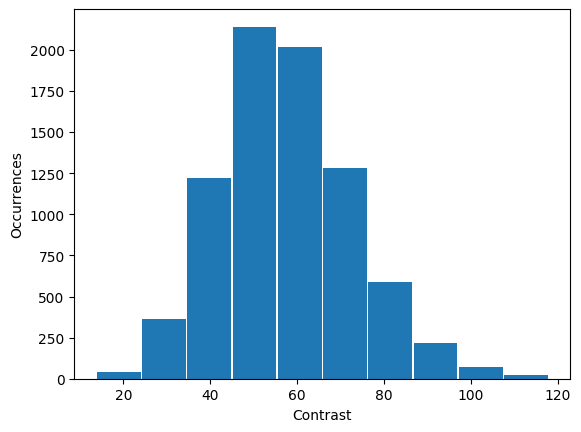
\includegraphics{images/graphs/test-contrast-hist.png}
    \caption{Contrast distribution of the images in the test dataset.}
    \label{fig:contrast:testing}
\end{figure}

\subsection{Bad quality images}

Within all the available images, some were really unusual, what could cause issues for participants to deal with. Malek Badreddine~\cite{badreddine2019bad}, who was a participant in the competition, found some examples of problematic images examples in the training dataset. These are shown in Figures \ref{fig:whale:0a5216ef5}, \ref{fig:whale:0c0bf8fb8}, \ref{fig:whale:0ce588f3d}, \ref{fig:whale:0d0a1d2fb}, \ref{fig:whale:0d7bd80d3}, \ref{fig:whale:0d25e3354}, \ref{fig:whale:0d605d56a}, \ref{fig:whale:0d37648f9}, \ref{fig:whale:0d757866b}, \ref{fig:whale:0db59bbec}, which are all classified as new whales. Another different example is the one shown in Figure \ref{fig:whale:0e6abdd05}, which is actually a whale drawing with a specified ID. In this case, at least, there were other ten pictures of the same whale available in the training set, what probably helped dealing with it. Interestingly, one of these ten images were also problematic, and illustrates the issue with poor photo angle (see Figure \ref{fig:whale:d6dce5f26}). % Check if there's a better way to reference all those images in a clearer way.

\begin{figure}
    \centering
    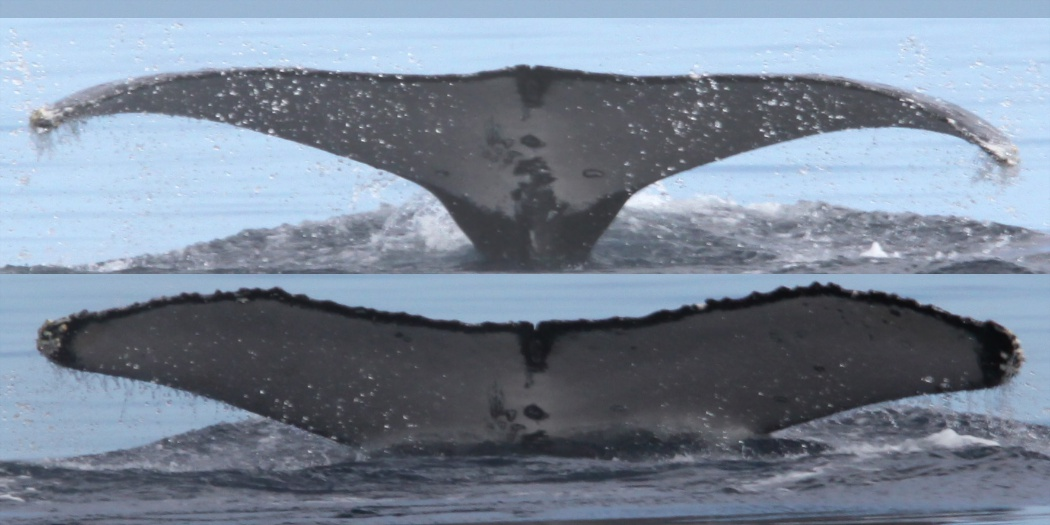
\includegraphics[width=0.95\textwidth]{images/whales/0a5216ef5.jpg}
    \caption{Two pictures of the same whale in the same image file.}
    \label{fig:whale:0a5216ef5}
\end{figure}

\begin{figure}
    \centering
    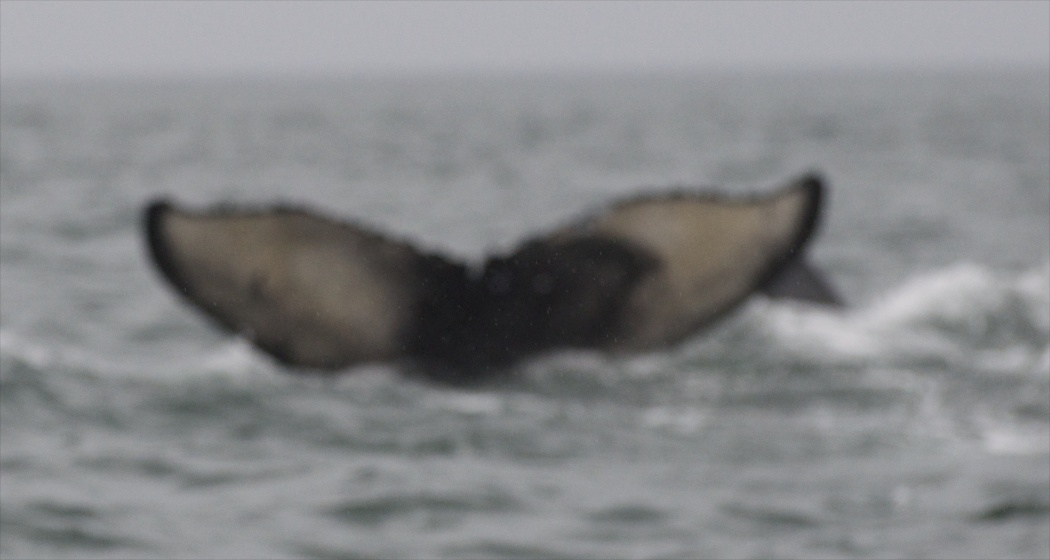
\includegraphics[width=0.95\textwidth]{images/whales/0c0bf8fb8.jpg}
    \caption{Example of very blurry image.}
    \label{fig:whale:0c0bf8fb8}
\end{figure}

\begin{figure}
    \centering
    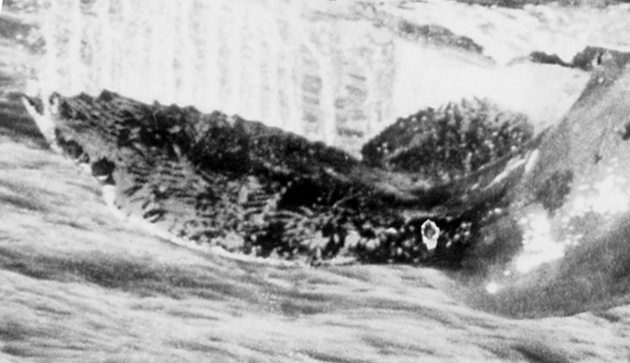
\includegraphics[width=0.95\textwidth]{images/whales/0ce588f3d.jpg}
    \caption{Picture of the front side markings of the fluke instead of the back side.}
    \label{fig:whale:0ce588f3d}
\end{figure}

\begin{figure}
    \centering
    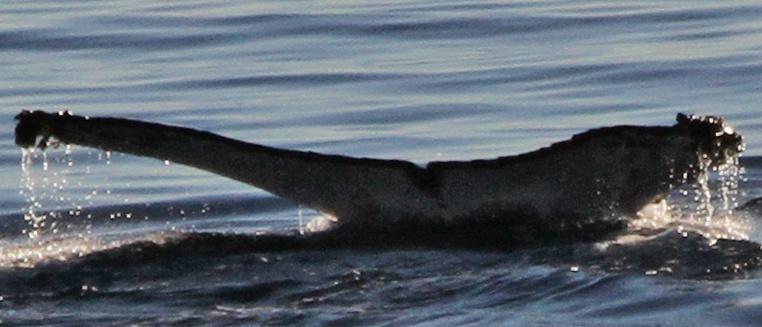
\includegraphics[width=0.95\textwidth]{images/whales/0d0a1d2fb.jpg}
    \caption{Poor picture angle.}
    \label{fig:whale:0d0a1d2fb}
\end{figure}

\begin{figure}
    \centering
    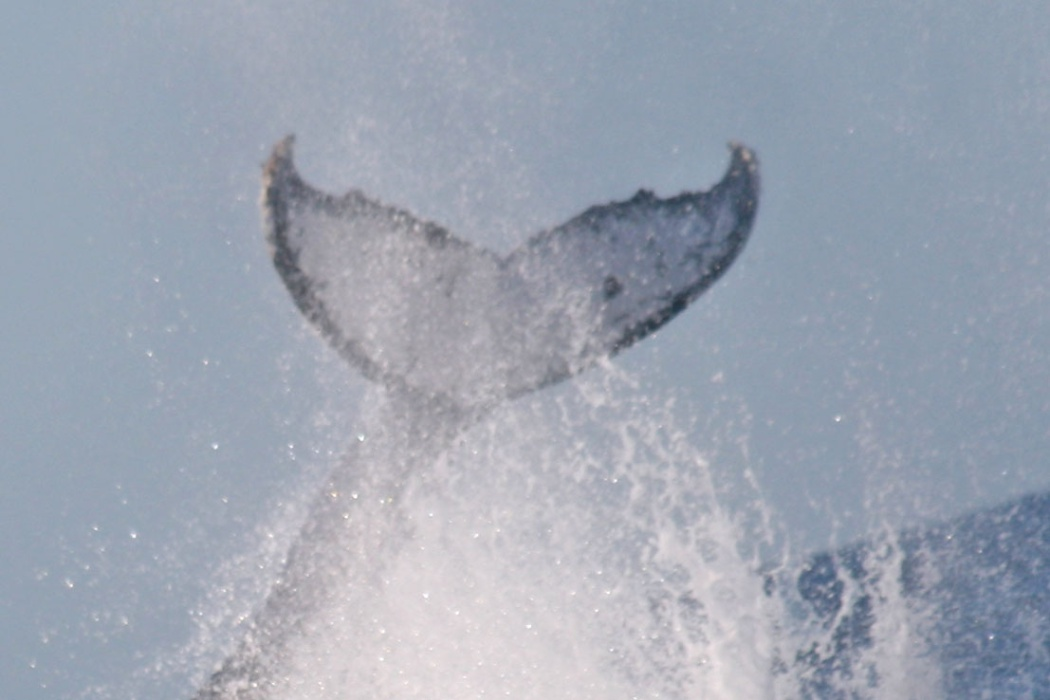
\includegraphics[width=0.95\textwidth]{images/whales/0d7bd80d3.jpg}
    \caption{Whale's tail occluded by a water spray.}
    \label{fig:whale:0d7bd80d3}
\end{figure}

\begin{figure}
    \centering
    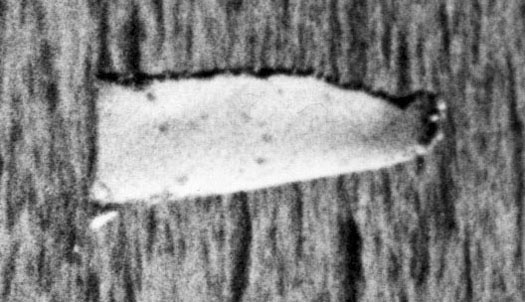
\includegraphics[width=0.95\textwidth]{images/whales/0d25e3354.jpg}
    \caption{Noisy image and only half of the fluke exposed in the image.}
    \label{fig:whale:0d25e3354}
\end{figure}

\begin{figure}
    \centering
    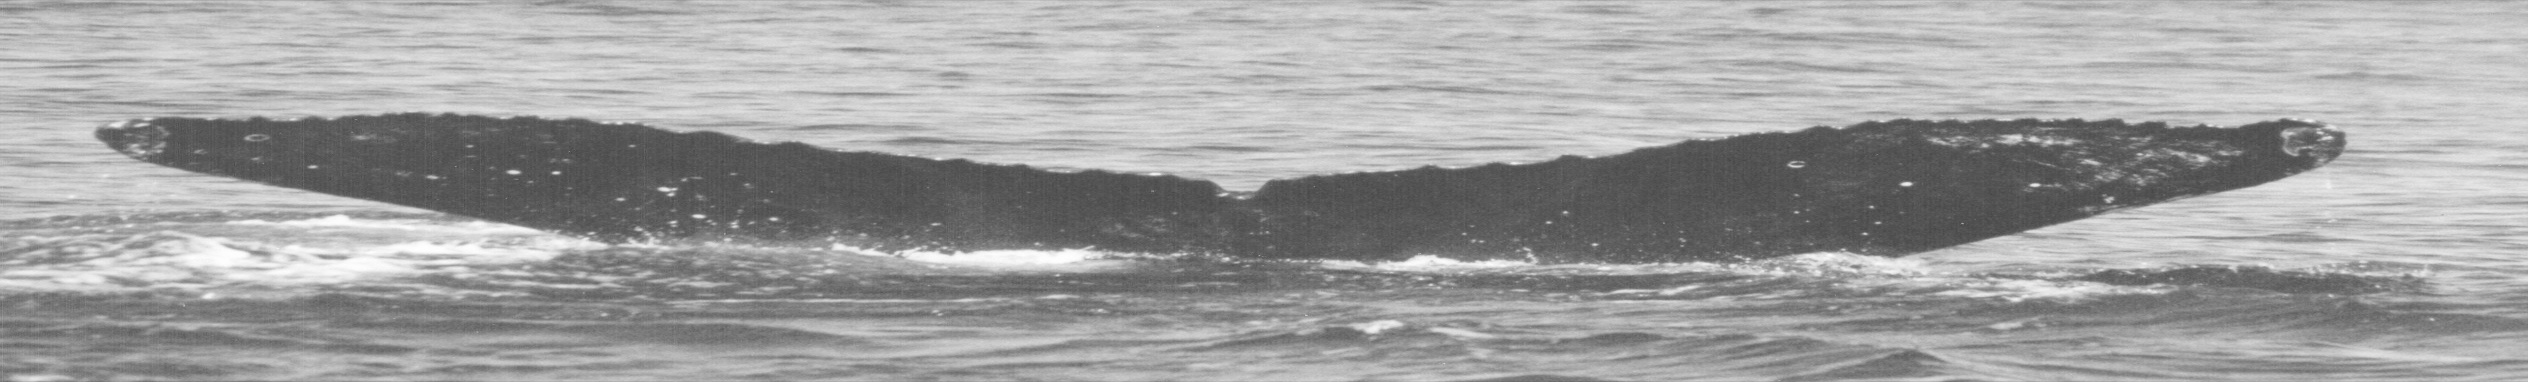
\includegraphics[width=0.95\textwidth]{images/whales/0d605d56a.jpg}
    \caption{Wrong aspect ratio ($2528 \times 382\: px$).}
    \label{fig:whale:0d605d56a}
\end{figure}

\begin{figure}
    \centering
    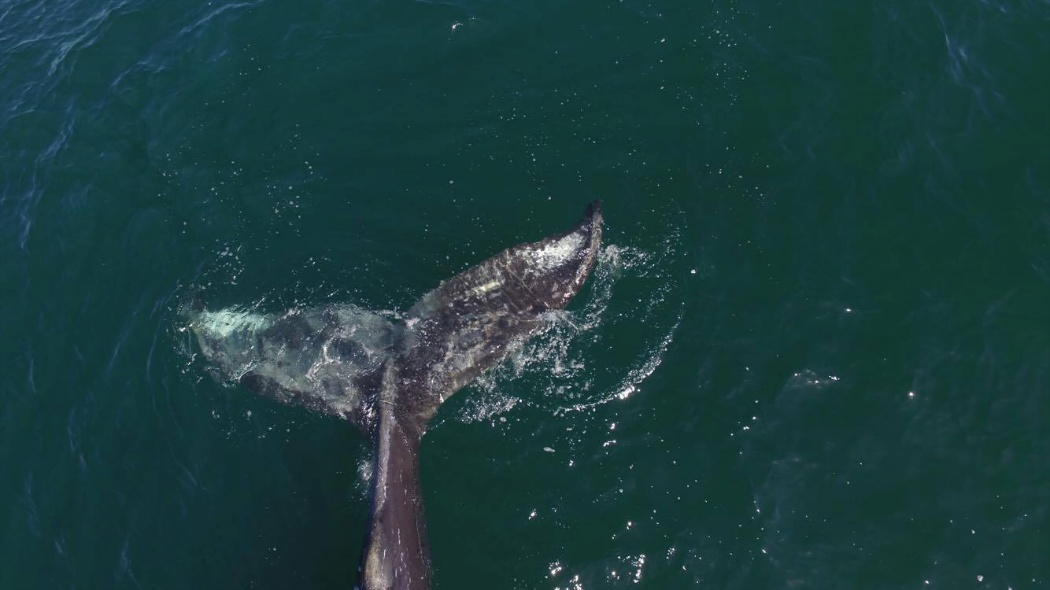
\includegraphics[width=0.95\textwidth]{images/whales/0d37648f9.jpg}
    \caption{Front side of the fluke instead of the back, and partially occluded by water.}
    \label{fig:whale:0d37648f9}
\end{figure}

\begin{figure}
    \centering
    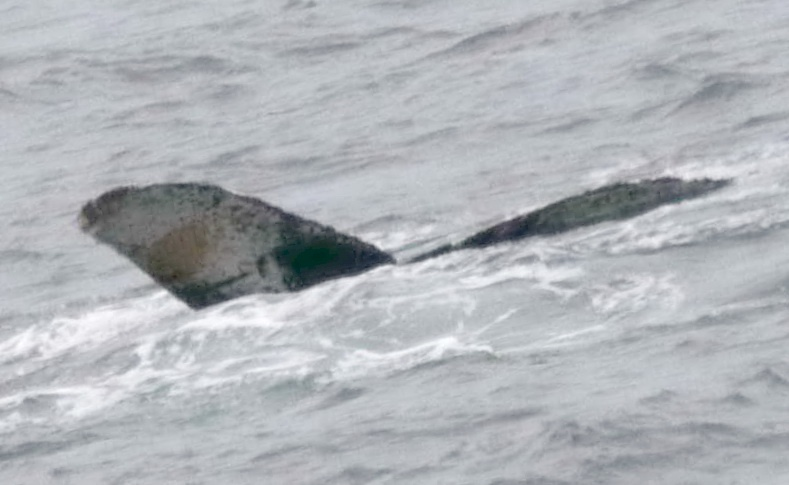
\includegraphics[width=0.95\textwidth]{images/whales/0d757866b.jpg}
    \caption{Partial occlusion of the tail, due to being half underwater.}
    \label{fig:whale:0d757866b}
\end{figure}


\begin{figure}
    \centering
    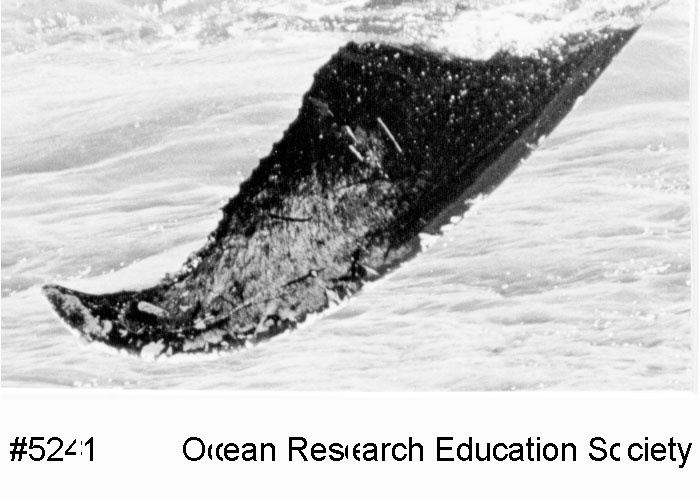
\includegraphics[width=0.95\textwidth]{images/whales/0db59bbec.jpg}
    \caption{Partially occluded and with text in the image.}
    \label{fig:whale:0db59bbec}
\end{figure}

\begin{figure}
    \centering
    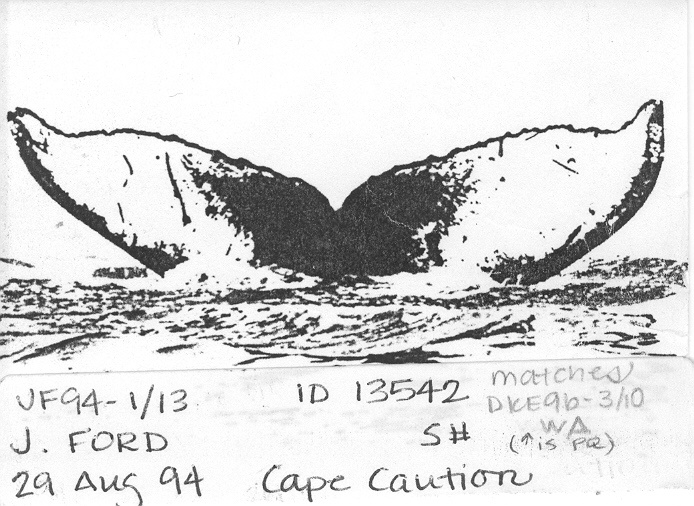
\includegraphics[width=0.95\textwidth]{images/whales/0e6abdd05.jpg}
    \caption{Whale sketch with handwriting.}
    \label{fig:whale:0e6abdd05}
\end{figure}

\begin{figure}
    \centering
    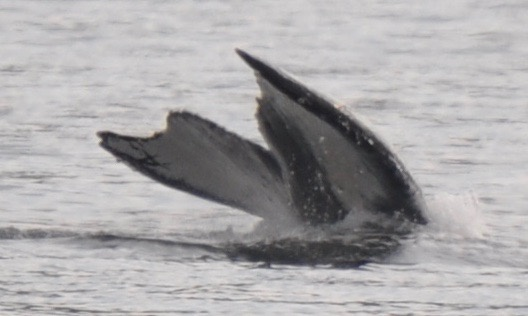
\includegraphics[width=0.95\textwidth]{images/whales/d6dce5f26.jpg}
    \caption{Problematic photo angle of the same whale that was sketched.}
    \label{fig:whale:d6dce5f26}
\end{figure}

\bibliographystyle{alpha}
\bibliography{references}

\end{document}
